\documentclass[12pt]{book}


\usepackage[dvips,letterpaper,margin=0.75in,bottom=0.75in]{geometry}
\usepackage{cite}
\usepackage{slashed}
\usepackage{graphicx}
\usepackage{amsmath}

\usepackage[american,fulldiode]{circuitikz}
\tikzset{component/.style={draw,thick,circle,fill=white,minimum size =0.75cm,inner sep=0pt}}

\begin{document}
\ctikzset{bipoles/thickness=1}
\ctikzset{bipoles/length=.6cm}

\title{Physics 80 Lab Manual}

\maketitle

\chapter{DC Circuits}

\section{Introduction}

In this lab, you will learn how to use your digital multimeter (DMM) and bench-top DC power supply to explore DC circuits involving resistors.  You will experimentally verify Ohm's law and the equivalent resistance for resistors in series and parallel.  You will solder two resistor circuits to explore the $\Delta$-$Y$ transformation for three terminal networks.

\section{Verification of Ohm's Law}

Build the circuit in Fig.~\ref{fig:ohmslaw}.

Discuss adjustment of current limit feature in the DC power supply.

\begin{figure}[htbp]
\begin{center}
\begin{tabular}{c@{\hskip 2cm}c}

\begin{circuitikz}[line width=1pt]
\draw (0,0) to[battery1,bipoles/length=1.5cm] ++(0,+4.0) to[short] ++(2.0,0) coordinate(A);
\draw (A) to[resistor,l_=$R_1$] ++(0,-2.0) to[short] ++(0,-2.0) to[short] ++(-2,0);
%node[ground,yscale=2.0]{};
\draw (0,1.7) node[left]{$-$};
\draw (0,2.4) node[left]{$+$};
\draw (A) to[short,*-] ++(2.0,0.0) to[short] ++(0.0,-1.0) node[component]{V} to[short] ++(0.0,-1.0) to[short,-*] ++(-2.0,0);
\end{circuitikz} &

\begin{circuitikz}[line width=1pt]
\draw (0,0) to[battery1,bipoles/length=1.5cm] ++(0,+4.0) to[short] ++(2.0,0);
\draw (A) to[resistor,l_=$R_1$] ++(0,-2.0) to[short] ++(0,-1.0) 
node[component]{A} to[short] ++(0,-1.0) to[short] ++(-2.0,0);
%node[ground,yscale=2.0]{};
\draw (0,1.7) node[left]{$-$};
\draw (0,2.4) node[left]{$+$};
\end{circuitikz} \\

(a) & (b) \\
\end{tabular}
\caption{Circuits for verifying Ohm's law.}
\label{fig:ohmslaw}
\end{center}
\end{figure}

\section{Voltage Divider}
One circuit you will encounter again and again is the humble voltage divider circuit of Fig.~\ref{fig:dividers}a.  

Verify voltage drop across lower resistors...
Verity resistance by making current measurement...


\begin{figure}[htbp]
\begin{center}
\begin{tabular}{c@{\hskip 2cm}c}
\begin{circuitikz}[line width=1pt]
\draw (0,0) to[battery1,bipoles/length=1.5cm] ++(0,+4.0) to[short] ++(2.0,0);
\draw (A) to[resistor,l_=$R_1$] ++(0,-2.0) to[resistor,l_=$R_2$] ++(0,-2.0) to[short] ++(-2.0,0);
%node[ground,yscale=2.0]{};
\draw (0,1.7) node[left]{$-$};
\draw (0,2.4) node[left]{$+$};
\end{circuitikz} &

\begin{circuitikz}[line width=1pt]
\draw (0,0) to[battery1,bipoles/length=1.5cm] ++(0,+4.0) to[short] ++(2.0,0) coordinate(A);
\draw (A) to[resistor,l_=$R_1$] ++(0,-4.0) to[short] ++(-2,0);
%node[ground,yscale=2.0]{};
\draw (0,1.7) node[left]{$-$};
\draw (0,2.4) node[left]{$+$};
\draw (A) to[short,*-] ++(2.0,0.0) to[resistor,l_=$R_2$] ++(0.0,-4.0) to[short,-*] ++(-2.0,0);
\end{circuitikz} \\


(a) & (b) \\
\end{tabular}
\caption{Circuits for driving an LED (a) directly from the signal voltage and (b) using a diode switch.}
\label{fig:dividers}
\end{center}
\end{figure}


\section{$\Delta$-$Y$ transformation}

\begin{figure}[htbp]
\begin{center}
\begin{tabular}{c@{\hskip 2cm}c}
\begin{circuitikz}[line width=1pt]
\draw (0,0) coordinate(A);
\draw (A) to[R,l_=$R_1$,*-*] ++(0,2.0);
\draw (A) to[R,*-*] ++(-1.73,-1);
\draw (A) to[R,*-*] ++(1.73,-1);
\end{circuitikz} &
\begin{circuitikz}[line width=1pt]
\draw (0,2) to [R] (1.73,-1) to [R,*-] (-1.73,-1) to [R,*-*] (0,2);
\end{circuitikz} \\
(a) & (b) \\
\end{tabular}
\caption{Equivalent three-node circuits.}
\label{fig:deltay}
\end{center}
\end{figure}


\section{Additions}

Effect of resistance measurement with current in resistor?

Loading of circuit by DMM.

\section{Pre-lab Calculations}
\noindent
1) Calculate the expected gain for the circuit in Fig.~\ref{fig:follower}.   Assume the capacitance $C$ is infinitely large, so that you can neglect the voltage divider at the input.\\

\noindent
2) Calculate the expected gain for the circuit in Fig.~\ref{fig:amp}.  Assume the capacitance $C$ is infinitely large, so that you can neglect the voltage divider at the input.

\chapter{Thevenin Equivalent Circuits}

\begin{figure}[htbp]
\begin{center}
\begin{tabular}{c@{\hskip 2cm}c}
\begin{circuitikz}[line width=1pt]
\draw (0,0) to[battery1,bipoles/length=1.5cm] ++(0,2.0) coordinate(X) to[R,l=$R_2$,-*] ++(2.0,0);
\draw (X) to[R,l=$R_1$] ++(0,2.0) to[short,-*] ++ (2.0,0) coordinate(X) to[short,-o] ++ (1.0,0);
\draw (X) to[battery1,bipoles/length=1.5cm] ++(0,-2.0) to[R,l=$R_3$] ++(0,-2.0) coordinate(X)
to[short,*-o] ++ (1.0,0);
\draw(X) to[short] ++(-2.0,0);
\end{circuitikz} &
\begin{circuitikz}[line width=1pt]
\draw (0,0) coordinate(X) to[battery1,bipoles/length=1.5cm] ++(0,2.0) to[R,l=$R_{th}$,-*] ++(0,2.0)
to[short,-o] ++ (3.0,0);
\draw(X) to[short,-o] ++ (3.0,0);
\end{circuitikz} \\
(a) & (b) \\
\end{tabular}
\caption{The circuit (a) you will be building in lab and it's (b) Thevenin Equilvalent.}
\label{fig:deltay}
\end{center}
\end{figure}

\chapter{Alternating Current and Time Varying Signals}
\section{Introduction}
In this lab you will use two essential new pieces of lab equipment (scope and function generator) to study alternating current and time varying signals.

\section{Function Generator}

\begin{figure}[htbp]
\begin{center}
\begin{circuitikz}[line width=1pt]
\draw (0,0) to[sinusoidal voltage source,bipoles/length=1.5cm] ++(0,3.0) to[short] ++(2.0,0) coordinate(X) to[short,*-o] ++(1.0,0) node[right]{A};
\draw (X) to[R,-*] ++(0,-3.0) coordinate(X) to[short,-o] ++(1.0,0) node[right]{B};
\draw (X) to[short,-*] ++(-2.0,0) node[ground,yscale=2.0]{};
\end{circuitikz} 
\caption{A function generator driving a resistor.}
\label{fig:mycirc}
\end{center}
\end{figure}

\section{Oscilloscope}

\section{Lissajous Patterns}

\begin{figure}[htbp]
\begin{center}
\begin{circuitikz}[line width=1pt]
\draw (0,0) to[square voltage source,bipoles/length=1.5cm] ++(0,4.0) to[short] ++(2.0,0)
to[R,-*] ++(0,-2.0) coordinate(X) to[short,*-o] ++(1.0,0) node[right]{A};
\draw (X) to[C,-*] ++(0,-2.0) coordinate(X) to[short,-o] ++(1.0,0) node[right]{B};
\draw (X) to[short,-*] ++(-2.0,0) node[ground,yscale=2.0]{};
\end{circuitikz} 
\caption{A function generator driving a resistor.}
\label{fig:mycirc}
\end{center}
\end{figure}

\chapter{RC and RL Transient Signals}

\chapter{Passive Filters and Resonance}
\section{Introduction}
In this lab you will use two essential new pieces of lab equipment (scope and function generator) to study the transient response of resistors and capacitors.

\section{RC Low-pass and High-pass Filters}

\begin{figure}[htbp]
\begin{center}
\begin{tabular}{c@{\hskip 2cm}c}

\begin{circuitikz}[line width=1pt]
\draw (0,0) to[sinusoidal voltage source,bipoles/length=1.5cm] ++(0,4.0) to[short] ++(2.0,0)
to[R,-*] ++(0,-2.0) coordinate(X) to[short,*-o] ++(1.0,0) node[right]{A};
\draw (X) to[C,-*] ++(0,-2.0) coordinate(X) to[short,-o] ++(1.0,0) node[right]{B};
\draw (X) to[short,-*] ++(-2.0,0) node[ground,yscale=2.0]{};
\end{circuitikz}  &

\begin{circuitikz}[line width=1pt]
\draw (0,0) to[sinusoidal voltage source,bipoles/length=1.5cm] ++(0,4.0) to[short] ++(2.0,0)
to[R,-*] ++(0,-2.0) coordinate(X) to[short,*-o] ++(1.0,0) node[right]{A};
\draw (X) to[C,-*] ++(0,-2.0) coordinate(X) to[short,-o] ++(1.0,0) node[right]{B};
\draw (X) to[short,-*] ++(-2.0,0) node[ground,yscale=2.0]{};
\end{circuitikz}  \\


(a) & (b) \\
\end{tabular}
\caption{A function generator driving a resistor.}
\label{fig:mycirc}
\end{center}
\end{figure}


\section{Resonant Band-pass Filter}

\begin{figure}[htbp]
\begin{center}

\begin{circuitikz}[line width=1pt]
\draw (0,0) to[sinusoidal voltage source,bipoles/length=1.5cm] ++(0,3.0) 
to[R,-*] ++(2.0,0) coordinate(X) to[short,*-*] ++(1.5,0) coordinate(Y) to[short,-o] ++(1.0,0) node[right]{A};
\draw (X) to[C,-*] ++(0,-3.0)  to[short,-*] ++(-2.0,0) node[ground,yscale=2.0]{};
\draw (Y) to[L,-*] ++(0,-3.0)  coordinate(X) to[short,-*] ++(-1.5,0);
\draw (X) to[short,-o] ++(1.0,0) node[right]{B};
\end{circuitikz}  
\caption{A function generator driving a resistor.}
\label{fig:mycirc}
\end{center}
\end{figure}

\chapter{The Diode}

\section{Introduction}

In this lab, you will measure the IV curve of a diode, use it to predict the operating point of a circuit, and use rectification to provide a DC current source with low ripple voltage.   In the process, you will learn how to use the Math mode of your scope to make a differential voltage measurement.

\section{Measuring the $I$-$V$ Curve of a Diode}

In this section you will measure the $I$-$V$ curve of a 1N914 diode, and compare your results to the curves available from the device data sheet.  To avoid taking a bunch of measurements by hand, we will use a trick to plot the curve directly on your oscilloscope using the XY mode.
\begin{figure}[htbp]
\begin{center}
\begin{tabular}{c@{\hskip 2cm}c}

\begin{circuitikz}[line width=1pt]
\draw
(0,0) to[sinusoidal voltage source,bipoles/length=1.5cm,l=$\tilde{V}$] (0,4) -- (2,4);
\draw
(2,4) node[right]{$P_2$} to[resistor,l=$R_1$,o-o] (2,2) node[right] {$P_1$} to[diode,l=$D_1$,-o](2,0) node[right]{G}-- (0,0)
;
\draw (0,0) -- ++(0,0) node[ground,yscale=2.0]{};
\end{circuitikz} &

\begin{circuitikz}[line width=1pt]
\draw
(0,0) to[sinusoidal voltage source,bipoles/length=1.5cm,l=$\tilde{V}$] (0,4) -- (4,4);
\draw
(2,4) to[resistor,l_=$R_1$,*-o] (2,2) node[left]{$P_1$} node[right]{(Ch.1)} to[diode,l_=$D_1$,o-*] (2,0)
(4,4) to[diode,l=$D_2$,-o] (4,2) node[right] {$P_2$ (Ch.2)} to[resistor,l=$R_2$,-o](4,0) node[right]{G}-- (0,0)
;
\draw (2,0) -- ++(0,0) node[ground,yscale=2.0]{};
\end{circuitikz} \\
(a) & (b) \\
\end{tabular}
\caption{Diode circuits for (a) demonstrating rectification and (b) plotting the diode IV curve on your oscilloscope.}
\label{fig:diodecircuits}
\end{center}
\end{figure}

Consider (but don't build!) the circuit in Fig.~\ref{fig:diodecircuits}a.  The voltage between points $P_2$ and $P_1$ is proportional to the current passing through the diode, and the voltage between points $P_1$ and $G$ is the voltage across the diode.  So if we could display $P_2-P_1$ versus $P_1-G$ on your scope we could use this circuit.  Unfortunately, this is not possible on your scope, because (1) the only valid place to put the scope probe ground shield clips is at the point $G$ (Why?) and (2) you can only display Channel 1 versus Channel 2 in XY mode.   

The solution is to drive two copies of the diode in series resistor, with the component order reversed, as in Fig.~\ref{fig:diodecircuits}b.  This way, we can connect the probe ground shields as required at point $G$, put the voltage across the diode on scope Channel 1 by connecting the probe tip at $P_1$, and put the voltage across the resistor (proportional to current through the diode) on scope Channel 2 by connecting the probe tip at $P_2$.

Build the circuit in Fig.~\ref{fig:diodecircuits}b using a 1N914 fast switching diode for $D_1$ and $D_2$ and $R_1= R_2 = 10~{\rm k\Omega}$.  Set your function generator for high-impedance output, providing AC with peak to peak voltage of $20~\rm V$ at a frequency of $100~\rm Hz$.  Before switching to XY mode, make certain that your Channel 1 has no voltage offset (that is, zero voltage is located at the origin) or else your diode output voltage won't be calibrated properly in your output plot.   Once you set this, try not to adjust the offset of Channel 1 or you'll have to redo it!  To minimize noise, set the bandwidth limit ``On'' for both channels (this is available in the menu for each input channel as ``BW Limit'').

\begin{figure}[htbp]
\begin{center}
\begin{tabular}{c@{\hskip 2cm}c}
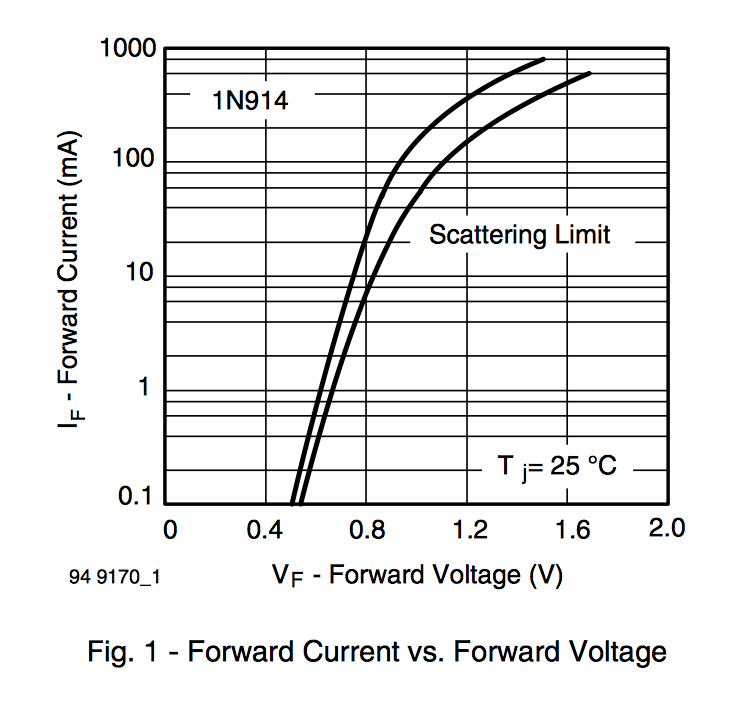
\includegraphics[height=0.25\textheight]{figs/1N914.png} &
\begin{picture}(200,100)
\put(0,0){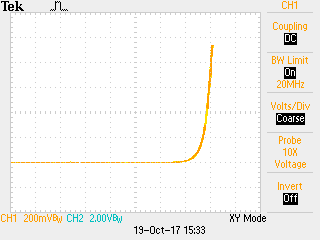
\includegraphics[height=0.25\textheight]{figs/diodeiv.png}}
\put(10,52){$0~mA$}
\put(10,70){$0.2~mA$}
\put(10,88){$0.4~mA$}
\put(10,106){$0.6~mA$}
\put(10,124){$0.8~mA$}
\put(10,142){$1.0~mA$}
\end{picture}\\
(a) & (b) \\
\end{tabular}
\caption{\label{fig:diodeiv} IV curves for the1N914 from (a) data sheet, and (b) as you will measure in this lab.  In the scope trace, the Channel 2 ($Y$) with scale set to $2~\rm V$ measures the voltage across a $10~\rm k\Omega$ resistor, so each division corresponds to $200~\rm \mu A$ as indicated. 
}
\end{center}
\end{figure}

Set the scope into XY mode, and see if you can reproduce the diode IV curve in Fig~\ref{fig:diodeiv}b.
Beats jotting down voltages in your logbook doesn't it?  Now jot down the voltage you expect across the diode for a current of $1~\rm mA$ in your logbook.  Where they overlap, does your measured IV curve agree with the curve from the component data sheet in Fig.~\ref{fig:diodeiv}a?

\section{Rectifying an AC Signal}

\begin{figure}[htbp]
\begin{center}
\begin{circuitikz}[line width=1pt]
\draw
(0,0) to[sinusoidal voltage source,bipoles/length=1.5cm,l=$\tilde{V}$] (0,4) -- (2,4)
(2,4) node[right]{$P_2$} to[diode,l=$D$,o-o] (2,2) node[right] {$P_1$} to[resistor,l=$R$,-o](2,0) node[right]{$G$} -- (0,0)
(2,0) -- ++(0,0) node[ground,yscale=2.0]{};
\end{circuitikz} 
\caption{A diode rectification circuit.}
\label{fig:rect}
\end{center}
\end{figure}

Set your function generator to provide an AC source with frequency $100~\rm Hz$ and peak-to-peak voltage $V_{\rm pp}=5~\rm V$.  Build the circuit in Fig.~\ref{fig:rect} using a 1N914 diode for $D$ and $R=1.8~\rm k\Omega$. 

With your scope probe ground shield clips both properly connected to the ground at $G$, monitor the voltage at points $P_1$ and $P_2$.   Sketch the voltage across the resistor $R$ and the voltage supplied by the function generator versus time on the same plot in your lab book. 

Using your scopes amplitude measurement feature, measure precisely (i.e. to within $50~\rm mV$ precision) the voltage drop across the diode at the peak current value, by measuring the difference between Channel 1 and Channel 2 of your scope at the peak.  Is this operating point consistent with your results from the previous section and the pre-lab calculations?

\section{Building a DC voltage source}

Now build the DC source circuit in Fig.~\ref{fig:fwrect} using a 1N914 diode for $D$ and $R_{\rm L}=18~\rm k\Omega$.  Adjust your function generator to provide a peak-to-peak voltage $V_{\rm pp} = 20~\rm V$.   

\begin{figure}[htbp]
\begin{center}
\begin{circuitikz}[line width=1pt]
\draw
(4,0) -- (0,0) node[left]{$G$} to[sinusoidal voltage source,l=$\tilde{V}$,bipoles/length=1.5cm,o-] (0,4) -- (4,4)
(2,2) to[diode,l_=D,-*] ++(0,-2) 
(2,2) to[diode,l=D,-*] ++(0,2) 
(4,4) to[diode,l_=D] ++(0,-2) 
(4,0) to[diode,l=D] ++(0,2)
(2,1.8) to[short,*-] ++(4,0) -- ++(0,-1.8) -- ++(2,0) coordinate (A)
(4,2.2) to[short,*-] ++(2,0) -- ++(0,1.8) -- ++(2,0) coordinate (B)
(B) -- ++(0,-1) coordinate (C)
(A) -- ++(0,1) node[right]{$P_1$} to[R,l=$R_{\rm L}$,o-o] (C) node[right]{$P_2$}
(2,0) -- ++(0,0) node[ground,yscale=2.0]{}
;
\end{circuitikz}
\caption{A full-wave rectifier.  Note that crossed lines without a dot are {\em not connected.}}
\label{fig:fwrect}
\end{center}
\end{figure}

To measure the performance of our DC source, we would like to measure the voltage across the resistor $R_L$ on the scope.  However, notice that the ground for the circuit is located at point $G$, so you cannot measure the voltage between $P_1$ and $P_2$ using a single probe.  To make the measurement, connect  both probe ground shield clips to the point $G$ as required, and connect the probe tips to points $P_1$ and $P_2$.  Next, use your scope's Math mode to subtract Channel 1 to from Channel 2.  The result of this operation is the voltage across the resistor $R_{\rm L}$.

Sketch the current as a function of time for a few cycles, and measure the amplitude.  In your lab report, explain the shape and the amplitude.

\section{Controlling the Ripple}

In class, we derived the following formula for the ripple voltage (the residual AC voltage after rectification) 
for a full-wave rectifier with a capacitance $C$:
\begin{displaymath}
\Delta V = \frac{I_{\rm max}}{2 f C}
\end{displaymath}
Add a capacitor with $C=1~\rm{\mu F}$ to your circuit, as in Fig.~\ref{fig:fwrectc} and sketch the resulting waveform for the voltage across the load resistor as measured with your scope.  Estimate the ripple voltage.  As your DMM is a handheld device that is not DC coupled, you may use it to measure the voltage across $R_L$ directly.  Using your DMM, measure the voltage across $R_L$ in both AC and DC mode.   How does the AC measurement relate to the ripple voltage $\Delta V$?  How do you various measurements compare to the voltages you calculated in pre-lab calculations?

For the last tweak, you are going to use a large electrolytic capacitor.  {\bf These capacitors are polarized, and will likely ``let the smoke out'' if you install them the wrong way.}  Making sure the negative terminal is connected as indicated in Fig.~\ref{fig:fwrectc}, install a $C=100~\rm \mu F$ electrolytic capacitor in your circuit and measure the ripple voltage.

\begin{figure}[htbp]
\begin{center}
\begin{circuitikz}[line width=1pt]
\draw
(4,0) -- (0,0) node[left]{$G$} to[sinusoidal voltage source,l=$\tilde{V}$,bipoles/length=1.5cm,o-] (0,4) -- (4,4)
(2,2) to[diode,l_=D,-*] ++(0,-2) 
(2,2) to[diode,l=D,-*] ++(0,2) 
(4,4) to[diode,l_=D] ++(0,-2) 
(4,0) to[diode,l=D] ++(0,2)
(2,1.8) to[short,*-] ++(4,0) -- ++(0,-1.8) -- ++(2,0) coordinate (D)
(4,2.2) to[short,*-] ++(2,0) -- ++(0,1.8) -- ++(2,0) coordinate (E)
(D) to[pC,l=$C$] (E)
(D) to[short,*-] ++(2,0) coordinate (A)
(E) to[short,*-] ++(2,0) coordinate (B)
(B) -- ++(0,-1) coordinate (C)
(A) -- ++(0,1) node[right]{$P_1$} to[R,l=$R_{\rm L}$,o-o] (C) node[right]{$P_2$}
(2,0) -- ++(0,0) node[ground,yscale=2.0]{}
;
\end{circuitikz}
\caption{A full-wave rectifier with ripple voltage limiting capacitor.  When using a polarized electrolytic capacitor, make certain that the negative terminal is connected to the lower half of the figure, as indicated.
}
\label{fig:fwrectc}
\end{center}
\end{figure}


\end{document}
